\documentclass{report}

\input{~/dev/latex/template/preamble.tex}
\input{~/dev/latex/template/macros.tex}

\title{\Huge{}}
\author{\huge{Nathan Warner}}
\date{\huge{}}
\pagestyle{fancy}
\fancyhf{}
\lhead{Warner \thepage}
\rhead{}
% \lhead{\leftmark}
\cfoot{\thepage}
\setborder
% \usepackage[default]{sourcecodepro}
% \usepackage[T1]{fontenc}

\begin{document}
    % \maketitle
        \begin{titlepage}
       \begin{center}
           \vspace*{1cm}
    
           \textbf{Chapters 1-4}
    
           \vspace{0.5cm}
           Stat 128: Elementary Statistics
            
                
           \vspace{1.5cm}
   
           A Document By: \\
           \textbf{Nathan Warner}
    
           \vfill
                
                
           \vspace{0.8cm}
         
           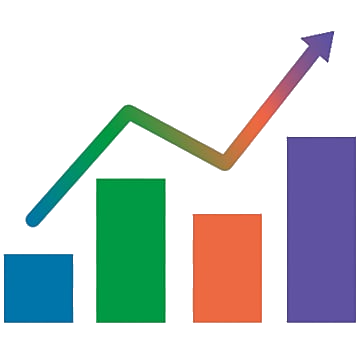
\includegraphics[width=0.4\textwidth]{./figures/2.png}
           \bigbreak \noindent 
            July 03, 2023  \\
           Computer Science \\
           Joliet Junior College \\
           United States\\
           
                
       \end{center}
    \end{titlepage}
    \tableofcontents
    \pagebreak \bigbreak \noindent
    \section{Learning Outcomes}
    \bigbreak \noindent 
    \textbf{Chapter 1:}
    \begin{enumerate}
        \item Define data collection techniques including observational studies and design of experiments.
        \item Identify appropriate sampling methods.
    \end{enumerate}
    \bigbreak \noindent 
    \textbf{Chapter 2:}
    \begin{enumerate}
        \item Differentiate qualitative and quantitative data graphically.  This includes graphs such as bar plots, histograms, and dot plots.
    \end{enumerate}
    \bigbreak \noindent 
    \textbf{Chapter 3:}
    \begin{enumerate}
        \item Calculate measures of central tendency for data.
        \item Explain the concept of resistance.
        \item Decide which measure of central tendency to report for various data sets.
        \item Determine measures of dispersion for data.
        \item Determine standard scores, percentiles, and quartiles.
        \item Identify outliers using quartiles.
        \item Interpret boxplots.
    \end{enumerate}
    \bigbreak \noindent 
    \textbf{Chapter 4:}
    \begin{enumerate}
        \item Evaluate the linear correlation coefficient for bivariate quantitative data.
        \item Evaluate whether the coefficient is significant at a given level.
        \item Explain the difference between correlation and causation.
        \item Determine the least-squares regression equation for a given set of bivariate data.
        \item Predict values of the dependent variable using the least-squares regression equation.
        \item Interpret the slope and intercept of the least-squares regression equation.
        \item Test the requirements of the least-squares regression model using residual analysis.
        \item Determine and interpret the coefficient of determination.
        \item Graphically analyze bivariate quantitative data for outliers and influential observations.
        \item Describe the association between two qualitative variables using conditional distributions.
        \item Explain Simpson’s Paradox.
    \end{enumerate}

    \pagebreak \bigbreak \noindent
    \section{Chapter 1:}

    \bigbreak \noindent 
    \subsection{1.1: Introduction to the Practice of Statistics}

    \bigbreak \noindent 
    \textbf{\textit{\underline{Objectives for this section.}}}
    \begin{enumerate}
        \item Define Statistics and Statistical Thinking
        \item Explain the Process of Statistics
        \item Distinguish between Qualitative and Quantitative Variables
        \item Distinguish Between Discrete and Continuous Variables.
    \end{enumerate}
    
    \bigbreak \noindent \bigbreak \noindent 
    \textbf{\textit{\underline{Define Statistics and Statistical Thinking:}}}
    \bigbreak \noindent
        Statistics is the science of collecting, organizing, summarizing, and analyzing information to draw conclusions or answer questions. In addition, statistics is about providing a measure of confidence in any conclusions.
        \bigbreak \noindent 
        \textbf{Note:} We must report a measure of our confidence in our results because we do not have 100\% certainty our answers are correct.
        \bigbreak \noindent 
        The information referred to in the definition above is \textit{data}. \textbf{Data} are a "fact or proposition used to draw a conclusion or make a decision." Data describes characteristics of an individual.
        \bigbreak \noindent 
        One crucial thing to understand about \textbf{data}, is that is \textbf{varies}. One thing that makes an interesting study is the fact that the data within the study varies. A study about number of hearts a human has is not only uninteresting but not worth doing. This is because the data does not vary.
        \bigbreak \noindent 
        \textbf{Two Major Goals:}
        \begin{enumerate}
            \item Describe Variability.
            \item Understand sources of Variability.
        \end{enumerate}
        \bigbreak \noindent 
        In Statistics, the same approach to solving a problem can still lead to different results. This does not happen in a math class.
        \vspace{1em}

        \bigbreak \noindent \bigbreak \noindent 
        \textbf{\textit{\underline{Explain the Process of Statistics.}}}
        \bigbreak \noindent 
        First lets define some vocabulary:
        \begin{itemize}
            \item \textbf{Population:} The entire group to be studied is called the population.
            \item \textbf{Sample:} In statistics, it is often impractical or impossible to get access to the entire \textbf{population}, which is why we only look at a \textbf{sample.} A sample is a \textbf{subset} of the population being studied.
            \item \textbf{Individual:} An individual is a person or object that is a member of the population being studied.
            \item \textbf{Statistic:} A statistic is a numerical summary of a sample.
            \item \textbf{Descriptive Statistics:} Descriptive statistics consist of organizing and summarizing data. Descriptive statistics describe data through numerical summaries, tables, and graphs.
            \item \textbf{Inferential Statistics:} inferential Statistics uses methods that take a result from a sample, extend it to the population, and measure the reliability of the result.
            \item \textbf{Parameter:} A parameter is a numerical summary of a population.
        \end{itemize}

        \bigbreak \noindent 
        \textbf{The process of statistics:}
        \begin{enumerate}
            \item Identify the problem to be solved. It is important to clearly lay out the questions that the researcher wants answered, along with clearly specifying which population the study applies.
            \item Collect the data.
            \item Describe the data.
            \item Preform inference.
        \end{enumerate}

        \bigbreak \noindent 
        \begin{mdframed}
          \textbf{Example: The AP - National Constitution Center conducted a national poll to learn how adult Americans feel existing gun-control laws infringe on the second amendment to the U.S Constitution}
          \bigbreak \noindent 
          \textbf{The Following statistical process allowed the researchers to conduct their study.}
          \begin{enumerate}
              \item \textbf{Identify the research objective.}: The researchers wished to determine the percentage of adult Americans who believe gun-control laws infringe on the public's right to bear arms.
            \item \textbf{Collect the information needed to answer the question posed in (1).}: It is unreasonable to expect to survey the more than 200 million adult Americans to determine how they feel about gun-control laws. So the researchers surveyed a sample of 1007 adult Americans. Of those surveyed, 514 stated they believe existing gun-control laws infringe on the public's right to bear arms.
            \item \textbf{Describe the data.}: Of the 1007 individuals in the survey, 51\% believe existing gun-control laws inferring on the public's right to bear arms. This is a descriptive statistic, because its value is determined from a sample.
            \item \textbf{Preform inference.}: The researchers at the AP - National Constitution Center wanted to extend the results of the survey to \textbf{all} adult Americans. When generalizing results from a sample to a population, the results are \textbf{uncertain}. To account for this uncertainty, researchers reported a 3\% \textit{margin of error.} This means that the researchers feel fairly certain (in fact, 95\% certain) that the percentage of \textit{all} adult Americans who believe existing gun-control laws infringe on the public's right to bear arms is somewhere between 48\% and 54\%

          \end{enumerate}
          
        \end{mdframed}

        \bigbreak \noindent \bigbreak \noindent 
        \textbf{\textit{\underline{Distinguish between Qualitative and Quantitative Variables}}}
        \bigbreak \noindent 
        First let's define some vocab:
        \begin{itemize}
            \item \textbf{Variables:} The characteristics of the individuals in a study. Variables vary, which means they can take on different values.
            \item \textbf{Constants:} Variables that do not vary. Inferential statistics is not necessary with constants.
        \end{itemize}
        \bigbreak \noindent 
        One goal of research is to learn the causes of variability.
        \bigbreak \noindent 
        Variables can be classified into two groups: qualitative and quantitative.
        \begin{itemize}
            \item \textbf{Qualitative, or categorical variables} allow for the classification of individuals base on some attribute or characteristic.
            \item \textbf{Quantitative variables} provide numerical measures of individuals. The values of a quantitative variable can be added or subtracted and provide meaningful results.
        \end{itemize}
        \bigbreak \noindent 
        \begin{mdframed}
          \textbf{Example: Determine whether the following variables are qualitative or quantitative.}
          \begin{enumerate}[label=\alph*.)]
              \item \textbf{Gender.}: Qualitative
              \item \textbf{Temperature.}: Quantitative
              \item \textbf{Number of days during the past week that a college student studied.}: Quantitative
              \item \textbf{Zip Code.} Qualitative
          \end{enumerate}
          \textbf{Caution:} A numeric value does not automatically suggest a variable is quantitative.
        \end{mdframed}

        \bigbreak \noindent 
        \textbf{\textit{\underline{Distinguish between Discrete and Continuous Variables.}}}
        \begin{itemize}
            \item A \textbf{discrete variable} is a quantitative variable that has either a finite number of possible values or a countable number of possible values. A discrete variable cannot take on every possible value between any two possible values.
            \item A \textbf{continuous variable} is a quantitative variable that has an infinite number of possible values that are not countable. A continuous variable may take on every possible value between any two values. Continuous variables typically result from measurement. Continuous variables are often rounded. If a certain make of car gets 24 miles per gallon (mpg) of gasoline, its miles per gallon must be greater than or equal to 23.5 and less than 24.5, or $23.5 \leq mpg \leq 24.5$
        \end{itemize}

        \bigbreak \noindent 
        This Figure illustrates the relationship among qualitative, quantitative, discrete, and continuous variables.

        \begin{figure}[ht]
            \centering
            \incfig{graph1}
            \label{fig:graph1}
        \end{figure}

        \bigbreak \noindent 
        \begin{mdframed}
          \textbf{Example: Distinguish whether the quantitative variables are discrete or continuous.}
          \begin{enumerate}[label=\alph*.)]
            \item \textbf{The number of heads obtained after flipping a coin five times.}: Discrete
            \item \textbf{The number of cars that arrive at a McDonald's drive through between 12:00 PM and 1:00 PM}: Discrete
            \item \textbf{The Distance a 2011 Toyota Prius can travel in city driving conditions with a full tank of gas.}: Continuous
          \end{enumerate}
        \end{mdframed}

        \bigbreak \noindent 
        \textbf{Vocab:}
        \begin{itemize}
            \item The list of observed values for a variable is \textbf{data.}
            \item \textbf{Qualitative data} are observations corresponding to a \textbf{qualitative variable.}
            \item \textbf{Quantitative data} are observations corresponding to a quantitative variable.
            \item \textbf{Discrete data} are observations corresponding to a discrete variable.
            \item \textbf{Continuous data} are observations corresponding to a continuous variable.
        \end{itemize}

        \bigbreak \noindent 
        \begin{mdframed}
          \textbf{Example: Distinguish between Variables and Data}
          \bigbreak \noindent 
          The following table presents a group of selected countries and information regarding these countries.
          \bigbreak \noindent 
          Identify the individuals, variables, and data.
          \begin{center}
              \begin{tabular}{|l|c|c|c|}
              \hline
              Country & Government Type & Life Expectancy (Years) & Population (in millions) \\
              	\hline
              Australia & Federal parliamentary democracy & 81.63 & 21.3   \\
              	\hline
            Canada & Constitutional monarchy & 81.23 & 33.5 \\
            \hline
            France & Republic & 80.98 & 64.4 \\
            \hline
            Morocco & Constitutional monarchy & 75.47 & 31.3 \\
            \hline
            Poland & Republic & 75.63 & 38.5 \\
            \hline
            Sri Lanka & Republic & 75.14 & 21.3\\
            \hline
            United States & Federal Republic & 78.11 & 307.2 \\
            \hline
              \end{tabular}
          \end{center}
          \bigbreak \noindent 
          \textbf{Qualitative}: Government Type \\
          \textbf{Quantitative}: Life Expectancy and Population \\
          \textbf{Continuous}: Life Expectancy \\
          \textbf{Discrete}: Population \\
          \textbf{Data}: Everything under Government Type, Life Expectancy, and Population.
      \item 
        \end{mdframed}

        \pagebreak \bigbreak \noindent
        \begin{center}
            \begin{large}
                \textbf{All Vocab / Concepts From Section 1.1}
            \end{large}
        \end{center}
        \line(1,0){490}
        \begin{itemize}
            \item \textbf{Population:} The entire group to be studied is called the population.
            \item \textbf{Sample:} In statistics, it is often impractical or impossible to get access to the entire \textbf{population}, which is why we only look at a \textbf{sample.} A sample is a \textbf{subset} of the population being studied.
            \item \textbf{Individual:} An individual is a person or object that is a member of the population being studied.
            \item \textbf{Statistic:} A statistic is a numerical summary of a sample.
            \item \textbf{Descriptive Statistics:} Descriptive statistics consist of organizing and summarizing data. Descriptive statistics describe data through numerical summaries, tables, and graphs.
            \item \textbf{Inferential Statistics:} inferential Statistics uses methods that take a result from a sample, extend it to the population, and measure the reliability of the result.
            \item \textbf{Parameter:} A parameter is a numerical summary of a population.
            \item \textbf{Variables:} The characteristics of the individuals in a study. Variables vary, which means they can take on different values.
            \item \textbf{Constants:} Variables that do not vary. Inferential statistics is not necessary with constants.
            \item \textbf{Data:} The list of observed values for a variable.
            \item \textbf{Qualitative data} are observations corresponding to a \textbf{qualitative variable.}
            \item \textbf{Quantitative data} are observations corresponding to a quantitative variable.
            \item \textbf{Discrete data} are observations corresponding to a discrete variable.
            \item \textbf{Continuous data} are observations corresponding to a continuous variable.
        \end{itemize}

        \bigbreak \noindent 
        \textbf{Concepts:}
        \begin{itemize}
            \item Statistics and Statistical Thinking.
            \item Describe Variability
            \item Understand Sources of variability
            \item Statistical studies are concerned with both describing the variability in the data and understanding the sources of variability in data. Understanding the sources allows researchers to control it and reach better conclusions.
            \item The process of statistics
            \item Inferential/Descriptive Statistics
            \item Variables
                \begin{itemize}
                    \item Qualitative (Categorical) / Quantitative
                    \item Discrete / Continuous
                \end{itemize}
            \item Data
                \begin{itemize}
                    \item Qualitative (Categorical) / Quantitative
                    \item Discrete / Continuous
                \end{itemize}
        \end{itemize}

        \pagebreak \bigbreak \noindent
        \subsection{1.2: Observational Studies versus Designed Experiments}
        \bigbreak \noindent 
        \textbf{\textit{\underline{Objectives for this section.}}}
        \begin{enumerate}
            \item Distinguish between an Observational Study and a Designed Experiment
            \item Explain the Various Types of Observational Studies
        \end{enumerate}

        \bigbreak \noindent 
        \textbf{\textit{\underline{Distinguish between an Observational Study and a Designed Experiment}}}
        \begin{itemize}
            \item \textbf{Observational studies:} Observational studies involve observing and analyzing data collected from real-world settings without any intervention or manipulation by the researcher. Researchers passively observe and record information to identify correlations or associations between variables.
            \item \textbf{Designed experiments:} Designed experiments, also known as randomized controlled trials (RCTs), involve researchers actively manipulating variables and randomly assigning participants to different groups. This allows researchers to establish cause-and-effect relationships by comparing the effects of different interventions or treatments on the outcome of interest.
        \end{itemize}
        \bigbreak \noindent 
        \textbf{Vocab:}
        \begin{itemize}
            \item \textbf{Explanatory Variable:} An explanatory variable, also known as an independent variable or predictor variable, is a variable that is manipulated or controlled by researchers in an experiment or study. It is the variable that is hypothesized to have an impact on the outcome or dependent variable. 
            \item \textbf{Lurking variable}: An explanatory variable that was not considered in a study, but that affects the value of the response variable.
            \item \textbf{Response Variable}: The response variable, also known as the dependent variable or outcome variable, is the variable that is measured or observed to determine the effect or response of the explanatory variable(s). It is the variable that researchers are interested in studying or predicting. 
            \item \textbf{Confounding:} Occurs when the effects of two or more explanatory variables are not separated. Therefore, any relation that may exist between an explanatory variable and the response variable may be due to some other variable or variables not accounted for in the study.
            \item \textbf{Census:} List of individuals in a population along with certain characteristics of each individual.
        \end{itemize}

        \bigbreak \noindent 
        \nt{Is observational studies, we \textbf{are not} allowed to make statements of \textit{causality}, meaning we cannot say that changes in the explanatory variable \textit{cause} changes in the response variable. We can only say changes in the explanatory variable are associated with changes in the response variable.}

        \bigbreak \noindent 
        Why would we ever conduct an observational study if we cannot claim causation? Because it is often unethical to conduct a designed experiment.
        \bigbreak \noindent 
        Consider the link between smoking and lung cancer. In a designed experiment (on humans) to determine if smoking causes lung cancer, a researcher would divide a group of volunteers into two groups—Group 1 would smoke a pack of cigarettes every day for the next 10 years, and Group 2 would not smoke. Eating habits, sleeping habits, and exercise would be controlled so that the only difference between the two groups would be smoking. After 10 years, the experiment's researcher would compare the proportion of participants in the study who contract lung cancer in the smoking group with the nonsmoking group. If the two proportions differ significantly, it could be said that smoking causes lung cancer. This designed experiment controls many potential cancer-causing factors that would not be controlled in an observational study. However, it is an unethical experiment. Do you see why?
        \bigbreak \noindent Other reasons exist for conducting observational studies over designed experiments. An article in support of observational studies states, "Observational studies have several advantages over designed experiments, including lower cost, greater timeliness, and a broader range of patients." From Kjell Benson, BA, and Arthur J. Hartz, MD, PhD. "A Comparison of Observational Studies and Randomized Controlled Trials." 

        \bigbreak \noindent 
        In designed experiments, it is possible to have two explanatory variables in a study that are related to each other and related to the response variable. For example, suppose Professor Egner wanted to conduct an experiment in which she compared student success using online homework versus traditional textbook homework. To do the study, she taught her morning statistics class using the online homework and her afternoon class using traditional textbook homework. At the end of the semester, she compared the final exam scores for the online section to the textbook section. If the morning section had higher scores, could Professor Egner conclude that online homework is the cause of higher exam scores? Not necessarily. It is possible that the morning class had students who were more motivated. It is impossible to know whether the outcome was due to the online homework or to the time at which the class was taught. In this sense, we say that the time of day the class is taught is a confounding variable.

        \bigbreak \noindent 
        \textbf{Lurking Vs Confounding Variables:}
        \bigbreak \noindent 
        The big difference between lurking variables and confounding variables is that lurking variables are not considered in the study (for example, we did not consider lifestyle in the pneumonia study) whereas confounding variables are measured in the study (for example, we measured morning versus afternoon classes).
        \bigbreak \noindent 
        So lurking variables are related to both the explanatory and response variables, and this relation is what creates the apparent association between the explanatory variable and response variable in the study. For example, lifestyle (healthy or not) is associated with the likelihood of getting an influenza shot as well as the likelihood of contracting pneumonia or influenza.
        \bigbreak \noindent 
        A confounding variable is a variable in a study that does not necessarily have any association with the other explanatory variable but does have an effect on the response variable. Perhaps morning students are more motivated, and this is what led to the higher final exam scores, not the homework delivery system.
        \bigbreak \noindent 
        The bottom line is that both lurking variables and confounding variables can confound the results of a study, so a researcher should be mindful of their potential existence.

        \bigbreak \noindent \bigbreak \noindent 
        \textbf{\textit{\underline{Explain the Various Types of Observational Studies}}}
        \bigbreak \noindent 
        \begin{itemize}
            \item \textbf{Cross-sectional Studies:} Observational studies that collect information about individuals at a specific point in time, or over a very short period of time.
            \item \textbf{case-control Studies:} These studies are \textbf{retrospective,} meaning that they require individuals to look back in time or require the researcher to look at existing records. In case-control studies, individuals that have certain characteristics are matched with those that do not.
                \begin{itemize}
                    \item \textbf{Positive:} Control group allows for a comparison
                    \item \textbf{Negative:} Individuals must remember details
                    \item \textbf{Negative:} Records might not exist
                \end{itemize}
            \item \textbf{Cohort Studies:} A cohort study first identifies a group of individuals to participate in the study (cohort). The cohort is then observed over a period of time. Over this time period, characteristics about the individuals are recorded. Because the data is collected over time, cohort studies are \textbf{prospective.}
                \begin{itemize}
                    \item \textbf{Advantage:} Researcher does not need to rely on memory of study participants or existing records.
                    \item \textbf{Disadvantage:} Requires a lot of time.
                    \item \textbf{Disadvantage:} Could be expensive.
                \end{itemize}
        \end{itemize}

        \pagebreak \bigbreak \noindent
        \textbf{Is a designed experiment superior to an observational study? Not necessarily.}
        \begin{itemize}
            \item Because cross-sectional and case-control observational studies are relatively inexpensive, they allow researchers to explore possible associations prior to undertaking large cohort studies or designed experiments.
            \item It is not always possible to conduct an experiment. For example, we could not conduct an experiment to investigate the perceived link between high-tension wires and leukemia (on humans). Do you see why?
        \end{itemize}

        \pagebreak \bigbreak \noindent
        \subsection{1.3: Simple Random Sampling}
        \bigbreak \noindent 
        \textbf{\textit{\underline{Learning Objectives for this section.}}}
        \begin{enumerate}
            \item Obtain a simple random sample
        \end{enumerate}
        \bigbreak \noindent 
        \textbf{Vocab:}
        \begin{itemize}
            \item \textbf{Random Sampling:} The process of using chance to select individuals from a population to be included in the sample.
            \item \textbf{Simple Random Sampling:} A sample of size $n$  from a population of size $N $  is obtained through simple random sampling if every possible sample of size $n$  has an equal chance of occurring. The sample is then called a simple random sample.
                \begin{itemize}
                    \item $n < N $
                \end{itemize}
            \item \textbf{frame:} a list of all the individuals within the population.
        \end{itemize}

        \bigbreak \noindent 
        \nt{For the results of a survey to be reliable, the characteristics of the individuals in the sample must be representative of the characteristics of the individuals in the population. The key to obtaining a sample representative of a population is to let chance or randomness, rather than convenience, play a role in dictating which individuals are in the sample. If convenience is used to obtain a sample, the results of the survey are meaningless.}

        \bigbreak \noindent 
        \textbf{Recognizing a Convenience Sample and Its Limitations:}
        \bigbreak \noindent 
        Suppose that Gallup wants to know the proportion of adult Americans who consider themselves to be baseball fans. If Gallup obtained a sample by standing outside Fenway Park (home of the Boston Red Sox professional baseball team), the survey results are not likely to be reliable. Why? Clearly, the individuals in the sample do not accurately reflect the makeup of the entire population.
        \bigbreak \noindent 
        Suppose you wanted to learn the proportion of students on your campus who work. It might be convenient to survey the students in your statistics class, but do these students represent the overall student body? Does the proportion of freshmen, sophomores, juniors, and seniors in your class mirror the proportion of freshmen, sophomores, juniors, and seniors on campus? Does the proportion of males and females in your class resemble the proportion of males and females across campus? Probably not. What about evening (or day) students? For these (and many other) reasons, the convenient sample is not representative of the population, which means that any results reported from your survey are misleading.

        \bigbreak \noindent 
        \textbf{Effective Sampling Techniques:}
        \begin{enumerate}
            \item \textbf{Simple random sampling}
            \item \textbf{Stratified sampling}
            \item \textbf{Systematic sampling}
            \item \textbf{Cluster sampling}
        \end{enumerate}
        \bigbreak \noindent 
        These sampling methods are designed so that any selection biases the surveyor introduced (knowingly or unknowingly) during the selection process are eliminated. In other words, the surveyor does not have a choice as to which individuals are in the study. We will discuss simple random sampling in this section and the remaining three types of sampling in the next section.

        \bigbreak \noindent 
        \begin{mdframed}
          \textbf{Bonus: Consider a set of 5 possibilities A-E, and we want to determine the total number of combinations of selecting 3 letters:}
          \bigbreak \noindent 
          We can use the formula:
          \begin{align*}
              nCk = \frac{n!}{(k!(n-k)!)}
          .\end{align*}
          \bigbreak \noindent 
          Where $n $ is the total number of classes in the course list and $k$ is the number of classes to be chosen.
          \bigbreak \noindent 
          So we have $n =5$ and $k = 3$:
          \begin{align*}
                \frac{5!}{(3!(5-3)!)} \\
                = \frac{5!}{3! \cdot 2!}\\
                 = \frac{5 \cdot 4 \cdot 3!}{3! \cdot 2\cdot 1} \\
                 = \frac{5 \cdot 4}{2\cdot 1} \\
                 = \frac{20}{2} \\
                 = 10
          .\end{align*}
          \bigbreak \noindent 
          And we can calculate the chance over a certain event happening with:
          \begin{align*}
              Probablility = \frac{Number of Occurences}{Total Number of Occurences}
          .\end{align*}
        \end{mdframed}

        \bigbreak \noindent 
        \textbf{How do we select the individuals in a simple random sample?}
        \bigbreak \noindent 
        We could write the names of the individuals in the population on different pieces of paper and then select names from a hat. Often, however, the size of the population is so large that performing simple random sampling in this fashion is not practical.
        \bigbreak \noindent 
        Typically, each individual in the population is assigned a unique number between 1 and $N$, Where $N$ is the size of the population. Then $n $ distinct random numbers are selected, where $n $ is the size of the population
        \bigbreak \noindent 
        To number the individuals in the population, we need a \textbf{frame:} a list of all the individuals within the population.

        \bigbreak \noindent 
        \textbf{Obtaining a simple random sample with calculator (ti-84)}
        \bigbreak \noindent 
        The accounting firm of Senese and Associates has grown. To make sure their clients are still satisfied with the services they are receiving, the company decides to send a survey out to a simple random sample of 5 of its 30 clients.
        \bigbreak \noindent 
        So we need 5 unique random numbers from a range of 1-30. To do this in our ti-84 calculator:
        \begin{enumerate}
            \item Math $\rightarrow$ Prod $\rightarrow$ randIntNorep
            \item Syntax: randIntNoRep(\textit{lowerbound}, \textit{upperbound}, \textit{$n$}), where $n$ is the number of unique random numbers we must generate.
            \item Lower: 1
            \item Upper: 30
            \item $n$: 5
            \item Select Paste.
        \end{enumerate}

        \pagebreak \bigbreak \noindent
        \subsection{1.4: Other Effective Sampling Methods}
        \bigbreak \noindent 
        \textbf{\textit{\underline{Learning Objectives For This Section.}}}
        \begin{enumerate}
            \item \textbf{Obtain a Stratified Sample}
            \item \textbf{Obtain a Systematic Sample}
            \item \textbf{Obtain a Cluster Sample}
        \end{enumerate}
        \bigbreak \noindent 
        \textbf{Vocab:}
        \begin{itemize}
            \item \textbf{Stratified sample}: is obtained by dividing the population into nonoverlapping groups called strata and then obtaining a simple random sample from each stratum. The individuals within each stratum should be homogenous (similar) in some way.
                \begin{itemize}
                    \item Within Stratified samples, the number of individuals sampled from each stratum should be proportional to the size of the strata in the population.
                \end{itemize}
            \item \textbf{Systematic sample} is obtained by selecting every $k$th individual from the population. The first individual selected corresponds to a number between 1 and $k$
            \item \textbf{Cluster sample} is obtained by selecting all individuals within a randomly selected collection or group of individuals.
            \item \textbf{Convenience sample:} the individuals are easily obtained and not based on randomness.
        \end{itemize}
        \bigbreak \noindent 
        \textbf{\textit{\underline{Obtaining a Stratified Sample:}}}
        \bigbreak \noindent 
        Suppose Congress was considering a bill that abolishes estate taxes. In an effort to determine the opinion of her constituency, a senator asks a pollster to conduct a survey within her state.
        \bigbreak \noindent 
        The pollster may divide the population of registered voters within the state into three strata: Republican, Democrat, and Independent. This grouping makes sense because the members within each of the three parties may have similar opinions regarding estate taxes, but opinions among parties may differ. The main criterion in performing a stratified sample is that each group (stratum) must have a common attribute that results in the individuals being similar within the stratum.
        \bigbreak \noindent 
        An advantage of stratified sampling over simple random sampling is that it may allow fewer individuals to be surveyed while it obtains the same or more information. This result occurs because individuals within each subgroup have similar characteristics, so opinions within the group are not as likely to vary much from one individual to the next. In addition, a stratified sample guarantees that each stratum is represented in the sample.

        \bigbreak \noindent \bigbreak \noindent 
        \textbf{\textit{\underline{Obtaining a Systematic Sample:}}}
        \bigbreak \noindent 
        For example, to learn about the outcome of an election, a pollster might survey every tenth individual that leaves a polling place.
        \bigbreak \noindent 
        Because systematic sampling does not require a frame, it is a useful technique when you cannot gather a list of the individuals in the population. Also, systematic samples typically provide more information for a given cost than does simple random sampling. In addition, systematic sampling is easier to employ; so there is less likelihood of interviewer error occurring, such as selecting the wrong individual to be surveyed.

        \bigbreak \noindent 
        \textbf{Choosing a value for $k $}:
        \bigbreak \noindent 
        If the size of the population is unknown, there is no mathematical way to determine $k$
        \bigbreak \noindent 
        The value  of $k$ must be small enough to achieve our desired sample size.
        \bigbreak \noindent 
        The value of $k$ must be large enough to obtain a sample that is representative of the population.

        \bigbreak \noindent 
        \begin{mdframed}
            \textbf{Example:}
            Suppose we have a scenario where $k = 30$, and we want to start with individual 3 and select 40 individuals.
            \bigbreak \noindent 
            Firstly, we can observe that the sequence follows an arithmetic progression.
            \bigbreak \noindent 
            We can represent the sequence as:
            \bigbreak \noindent 
            \[a_{40} = \{3, 33, 63, \ldots, a_{40}\}\]
            \bigbreak \noindent 
            To find the 40th term, $a_{40}$, we can use the formula:
            \bigbreak \noindent 
            \[a_{n} = a + (n-1)d,\quad \text{where } n = 40,\ d = 30\]
            \bigbreak \noindent 
            Substituting the values into the formula:
            \bigbreak \noindent 
            \[a_{40} = 3 + (40-1) \cdot 30 = 1173\]
            \bigbreak \noindent 
            Therefore, our sequence is:
            \bigbreak \noindent 
            \[a_{40} = \{3, 33, 63, \ldots, 1173\}\]
            \bigbreak \noindent 
            \textbf{Note:} It's important to note that if our population does not have 1173 individuals, the desired sample size will not be achieved.
            \bigbreak \noindent 
        \end{mdframed}
        \bigbreak \noindent 
        \begin{mdframed}
          \textbf{Example: Now Suppose $k=4$}
          \bigbreak \noindent 
          \begin{align*}
              a_{40} = 3 + (40-1)\cdot 4 \\
              = 159
          .\end{align*}
          \bigbreak \noindent 
          So we have the sequence:
          \begin{align*}
              a_{40} = \{3,7,11,...,159\}
          .\end{align*}
          \bigbreak \noindent 
          \textbf{Note:} Suppose our population is Kroger shoppers, The $159^{th}$ shopper might leave the store at 3pm, so our survey would not include any of the evening shoppers.
        \end{mdframed}
        \bigbreak \noindent 
        \nt{An estimate of the size of the population would help to determine an appropriate value of $k $}

        \pagebreak \bigbreak \noindent
        \textbf{Systematic Sampling Determining $k$ when $N$ is Known:}
        \bigbreak \noindent 
        Steps to deduce $k$:
        \begin{enumerate}
            \item If possible, approximate the population size $N$. 
            \item Determine the sample size desired, $n$. 
            \item Divide $N$ by $n$ \bigg($\frac{N}{n},$\bigg) and round down to the nearest integer. This value is $k$.
            \item Randomly select a number between $1\ and\ k$, call this number $a$ (starting point)
            \item The sample will consist of the following individuals:
                \begin{align*}
                    a_{n} = a, a + k, a +2k,..., a + (n-1)k
                .\end{align*}
        \end{enumerate}
        \bigbreak \noindent 
        \begin{mdframed}
          \textbf{Example: Suppose $N=20,325$ and we desire a sample size of $n=100$. }
          \bigbreak \noindent 
          \begin{align*}
              K= \frac{20,325}{100} \\
              K= 203
          .\end{align*}
          \bigbreak \noindent 
          Now let's further suppose that we start with the $90^{th}$ individual. 
          \bigbreak \noindent 
          To compute our arithmetic sequence with these parameters, first lets find $a_{100}$:
          \begin{align*}
              a_{100} = 90 + (100-1)\cdot 203 \\
              a_{100} = 19890
          .\end{align*}
          \bigbreak \noindent 
          So we have the sequence:
          \begin{align*}
              a_{100} = \{90, 293, 496,...,20187\}
          .\end{align*}
        \end{mdframed}

        \pagebreak \bigbreak \noindent
        \textbf{\textit{\underline{Obtain a Cluster Sample.}}}
        \bigbreak \noindent 
        Suppose a school administrator wants to learn the characteristics of students enrolled in online classes. Rather than obtaining a simple random sample based on the frame of all students enrolled in online classes, the administrator treats each online class as a cluster and then finds a simple random sample of these clusters. The administrator then surveys all students in the selected clusters. This reduces the number of classes that get surveyed.
        \bigbreak \noindent 
        The following questions arise in cluster sampling:
        \begin{itemize}
            \item How do I cluster the population?
            \item How many clusters do I sample?
            \item How many individuals should be in each cluster?
        \end{itemize}
        \bigbreak \noindent 
        First, we must determine whether the individuals within the proposed cluster are homogeneous or heterogeneous.
        \bigbreak \noindent 
        city blocks tend to have similar households. Survey responses from houses on the same city block are likely to be similar. This results in duplicate information. We conclude that if the clusters have homogeneous individuals, it is better to have more clusters with fewer individuals in each cluster.
        \bigbreak \noindent 
        What if the cluster is heterogeneous? Under this circumstance, the heterogeneity of the cluster likely resembles the heterogeneity of the population. In other words, each cluster is a scaled-down representation of the overall population.
        \bigbreak \noindent 
        For example, a quality control manager might use shipping boxes that contain 100 light bulbs as a cluster. The manager does this because the rate of defects within the cluster resembles the rate of defects in the population, assuming that the bulbs are randomly placed in the box. Thus, when each cluster is heterogeneous, fewer clusters with more individuals in each cluster are appropriate.

        \bigbreak \noindent 
        \textbf{Convenience Sampling:}
        \bigbreak \noindent 
        In the four sampling techniques just presented (simple random sampling, stratified sampling, systematic sampling, and cluster sampling), the individuals are selected randomly. Often, however, inappropriate sampling methods are used in which the individuals are not randomly selected.
        \bigbreak \noindent 
        Have you ever been stopped in the mall by someone holding a clipboard? These folks are responsible for gathering information, but their methods of data collection are inappropriate, and the results of their analysis are suspect because they collect data using a convenience sample.
        \bigbreak \noindent 
        The most popular convenience samples are those in which the individuals in the sample are self-selected, meaning the individuals themselves decide to participate in the survey. Self-selected surveys are also called voluntary response samples. One example of self-selected sampling is phone-in polling—a radio personality will ask his or her listeners to phone or text the station to submit their opinions. Another example is the use of the Internet to conduct surveys. For example, a TV news show will present a story regarding a certain topic and ask its viewers to "tell us what you think" by completing an online questionnaire or tweeting an opinion with a hashtag.
        \bigbreak \noindent 
        Both of these samples are poor designs because the individuals who decide to be in the sample generally have strong opinions about the topic. A more typical individual in the population will not bother phoning, texting, or tweeting to complete a survey. Any inference made regarding the population from this type of sample should be made with extreme caution.

        \pagebreak \bigbreak \noindent
        \textbf{Multistage Sampling}
        \bigbreak \noindent 
        In practice, most large-scale surveys obtain samples using a combination of the techniques just presented.
        \bigbreak \noindent 
        As an example of multistage sampling, consider Nielsen Media Research. Nielsen randomly selects households and, through a People Meter, monitors the television programs these households are watching. The meter is an electronic box connected to each TV within the household. The People Meter measures what program is being watched and who is watching it. Nielsen selects the households with the use of a two-stage sampling process.
        \begin{enumerate}
            \item U.S. Census data, Nielsen divides the country into geographic areas (strata). The strata are typically city blocks in urban areas and geographic regions in rural areas. About 
            \item sends representatives to the selected strata and lists households within the strata. The households are then randomly selected through a simple random sample.
        \end{enumerate}
        Nielsen sells the information obtained to television stations and companies. These results are used to help determine prices for commercials.

        \bigbreak \noindent 
        \textbf{Sample Size Considerations:}
        \bigbreak \noindent 
        Throughout our discussion of sampling, we did not mention how to determine the sample size. Researchers need to know how many individuals they must survey to draw conclusions about the population within some predetermined margin of error.
        \bigbreak \noindent 
        Researchers must find a balance between the reliability of the results and the cost of obtaining these results. Time and money determine the level of confidence researchers will place on the conclusions drawn from the sample data. The more time and money researchers have available, the more accurate the results of the statistical inference will be.
        \bigbreak \noindent 
        Later in the course, we will discuss techniques for determining the sample size required to estimate characteristics regarding the population within some margin of error. (For a detailed discussion of sample size considerations, consult a text on sampling techniques such as Elements of Sampling Theory and Methods by Z. Govindarajulu, Pearson, 1999.)

        \pagebreak \bigbreak \noindent
        \subsection{1.5: Bias in Sampling}
        \bigbreak \noindent 
        \textbf{\textit{\underline{Learning Objectives For This Section:}}}
        \begin{enumerate}
            \item \textbf{Explain the Sources of Bias in Sampling}
        \end{enumerate}
        \bigbreak \noindent 
        \textbf{Vocab:}
        \begin{itemize}
            \item \textbf{Bias:} If the results of the sample are not representative of the population. Sampling bias means that the technique used to obtain the sample's individuals tends to favor one part of the  population over another. Any convenience sample has sampling bias because the individuals are not chosen through a random sample.
            \item \textbf{Undercoverage:} Occurs when the proportion of one segment of the population is lower in a sample than it is in the population. This can result if the frame used to obtain the sample is incomplete or not representative of the population.
            \item \textbf{Sampling bias:} sampling bias is a bias in which a sample is collected in such a way that some members of the intended population have a lower or higher sampling probability than others. It results in a biased sample of a population in which all individuals, or instances, were not equally likely to have been selected
            \item \textbf{Nonresponse bias:} exists when individuals selected to be in the sample who do not respond to the survey have different opinions from those who do
                \begin{itemize}
                    \item This can be controlled with \textbf{callbacks}.
                    \item This can also be controlled with \textbf{rewards or incentives}
                \end{itemize}
            \item \textbf{Response bias:} Exists when the answers on a survey do not reflect the true feelings of the respondent.
            \item \textbf{Open Question:} Allows the respondent to choose his or her response
            \item \textbf{Closed Question:} requires the respondent to choose from a list of predetermined responses
            \item \textbf{Nonsampling errors:} result from undercoverage, nonresponse bias, response bias, or data-entry error. Such errors could also be present in a census.
            \item \textbf{Sampling error:} results from using a sample to estimate information about a population. This type of error occurs because a sample gives incomplete information about a population.
        \end{itemize}
        \bigbreak \noindent 
        \textbf{\textit{\underline{Explain the sources of Bias in Sampling:}}}
        \bigbreak \noindent 
        There are three sources of bias in sampling:
        \begin{itemize}
            \item \textbf{Sampling bias}
            \item \textbf{Nonresponse bias}
            \item \textbf{Response bias}
        \end{itemize}
        \bigbreak \noindent 
        \textbf{Interviewer Error.}
        \bigbreak \noindent 
        Do not be quick to trust surveys conducted by poorly trained interviewers. 
        \bigbreak \noindent 
        Do not trust survey results if the sponsor has a vested interest in the results of the survey.
        \bigbreak \noindent 
        \textbf{Misrepresented Errors}
        \bigbreak \noindent 
        Some survey questions result in responses that misrepresent facts or are flat-out lies.
        \bigbreak \noindent 
        \textbf{Wording of Questions.}
        \bigbreak \noindent 
        The way a question is worded can lead to response bias in a survey, so questions must always be asked in balanced form.

        \bigbreak \noindent 
        \textbf{Ordering of Questions or Words}
        \bigbreak \noindent 
        Many surveys will rearrange the order of the questions within a questionnaire so that responses are not affected by prior questions.
        \bigbreak \noindent 
        \textbf{Type of Question.}
        \bigbreak \noindent 
        One of the first considerations in designing a question is determining whether the question should be \textit{open} or \textit{closed}
        \bigbreak \noindent 
        In closed questions, the possible responses should be rearranged because respondents are likely to choose early choices in a list rather than later choices.
        \bigbreak \noindent 
        Closed questions limit the number of respondent choices and, therefore, the results are mush easier to analyze. The limited choices, however, do not always include a respondent's desired choice.
        \bigbreak \noindent 
        An open question should be phrased so that the responses are similar. This allows for easy analysis of the responses
        \bigbreak \noindent 
        \nt{Survey designers recommend conducting pretest surveys with open questions and then using the most popular answers as the choices on closed-question surveys
            \\
            The goal is to limit the number of choices in a closed question without forcing respondents to choose an option they do not prefer, which would make the survey have response bias.
        }

        \bigbreak \noindent 
        \textbf{Can a census have bias? }
        \bigbreak \noindent 
        Yes.
        \bigbreak \noindent 
        A question on a census form could be misunderstood, thereby leading to response bias in the results.
        \bigbreak \noindent 
        We also mentioned that it is often difficult to contact each individual in a population. For example, the U.S. Census Bureau faces challenges in counting each homeless person in the country, so the census data published by the U.S. government likely suffers from nonresponse bias.

        \bigbreak \noindent 
        \textbf{Sampling Error versus Nonsampling Error:}
        \bigbreak \noindent 
        Nonresponse bias, response bias, and data-entry errors are types of nonsampling error.

        \bigbreak \noindent 
        However, when a sample is used to learn information about a population, sampling error is also likely to occur.
        \bigbreak \noindent 

        \pagebreak \bigbreak \noindent
        \subsection{1.6: The Design of Experiments}
        \bigbreak \noindent 
        \textbf{\textit{\underline{Learning Objectives For This Section:}}}
        \begin{enumerate}
            \item \textbf{Describe the Characteristics of an Experiment (vocab)}
            \item \textbf{Explain the Steps in Designing an Experiment}
            \item \textbf{Explain the Completely Randomized Design}
            \item \textbf{Explain the Matched-Pairs Design}
        \end{enumerate}
        \bigbreak \noindent 
        \textbf{Vocab:}
        \begin{itemize}
            \item \textbf{Experiment:} is a controlled study conducted to determine the effect of varying one or more explanatory variables or \textbf{factors} has on a response variable. 
            \item \textbf{Factor:} A variable whose effect on the response variable is to be assessed by the experimenter
            \item \textbf{Treatment:} Any combination of the values of the factors is called a treatment
            \item \textbf{Experimental Unit (or subject)} is a person, object or some other well-defined item upon which a treatment is applied
            \item \textbf{Control Group:} Serves as a baseline treatment that can be used to compare to other treatments.
            \item \textbf{Placebo:} is an innocuous medication, such as a sugar tablet, that looks, tastes, and smells like the experimental medication.
            \item \textbf{Blinding:} refers to nondisclosure of the treatment an experimental unit is receiving.
            \item \textbf{Single-blind} experiment is one in which the experimental unit (or subject) does not know which treatment he or she is receiving.
            \item \textbf{Double-blind} experiment is one in which neither the experimental unit nor the researcher in contact with the experimental unit knows which treatment the experimental unit is receiving.
            \item \textbf{Design:} To design an experiment means to describe the overall plan in conducting the experiment. Conducting an experiment requires a series of steps.
            \item \textbf{completely randomized design:} is one in which each experimental unit is randomly assigned to a treatment.
            \item \textbf{matched-pairs design:} is an experimental design in which the experimental units are paired up. The pairs are selected so that they are related in some way (that is, the same person before and after a treatment, twins, husband and wife, same geographical location, and so on). There are only two levels of treatment in a matched-pairs design.
        \end{itemize}

        \bigbreak \noindent 
        \textbf{\textit{\underline{Steps in Designing an Experiment:}}}
        \bigbreak \noindent 
        \begin{enumerate}
            \item Identify the Problem to Be Solved. The statement of the problem should be as explicit as possible and should provide the experimenter with direction. The statement must also identify the response variable and the population to be studied. Often, the statement is referred to as the claim.
            \item Determine the Factors That Affect the Response Variable. The factors are usually identified by an expert in the field of study. In identifying the factors, ask, “What things affect the value of the response variable?” After the factors are identified, determine which factors to fix at some predetermined level, which to manipulate, and which to leave uncontrolled.
            \item Determine the Number of Experimental Units. As a general rule, choose as many experimental units as time and money allow. Techniques exist for determining sample size, provided certain information is available.
            \item Determine the Level of Each Factor. There are two ways to deal with the factors, control or randomize.
                \begin{enumerate}
                    \item Control: There are two ways to control the factors.
                        \begin{enumerate}[label=\alph*.)]
                            \item Set the level of a factor at one value throughout the experiment (if you are not interested in its effect on the response variable).
                            \item Set the level of a factor at various levels (if you are interested in its effect on the response variable). The combinations of the levels of all varied factors constitute the treatments in the experiment.
                        \end{enumerate}
                    \item Randomize: Randomly assign the experimental units to treatment groups.  Because it is difficult, if not impossible, to identify all factors in an experiment, randomly assigning experimental units to treatment groups reduces the effect of variation attributable to factors (explanatory variables) not controlled. That is, randomly assigning experimental units to treatment groups tends to "even out" any uncontrolled factors.
                \end{enumerate}
            \item Conduct the Experiment.
                \begin{enumerate}[label=\alph*.)]
                    \item Replication occurs when each treatment is applied to more than one experimental unit. Using more than one experimental unit for each treatment ensures the effect of a treatment is not due to some characteristic of a single experimental unit. It is a good idea to assign an equal number of experimental units to each treatment.
                    \item Collect and process the data. Measure the value of the response variable for each replication. Then organize the results. The idea is that the value of the response variable for each treatment group is the same before the experiment because of randomization. Then any difference in the value of the response variable among the different treatment groups is a result of differences in the level of the treatment.
                \end{enumerate}
            \item Test the Claim. This is the subject of inferential statistics. Inferential statistics is a process in which generalizations about a population are made on the basis of results obtained from a sample. Provide a statement regarding the level of confidence in the generalization.
        \end{enumerate}

        \bigbreak \noindent 
        \textbf{\textit{\underline{Explain a Matched-Pairs Design:}}}
        \bigbreak \noindent 
        In matched-pairs design, one matched individual will receive one treatment and the other receives a different treatment. The matched pair is randomly assigned to the treatment using a coin flip or a random-number generator. We then look at the difference in the results of each matched pair. One common type of matched-pairs design is to measure a response variable on an experimental unit before and after a treatment is applied. In this case, the individual is matched against itself. These experiments are sometimes called before–after or pretest–posttest experiments.

        \pagebreak \bigbreak \noindent
        \section{Chapter 2:}
        \bigbreak \noindent 
        \subsection{2.1: Organizing Qualitative Data}
        \bigbreak \noindent 
        \textbf{\textit{\underline{Learning Objectives for This Section:}}}
        \begin{enumerate}
            \item \textbf{Organize Qualitative Data in Tables}
            \item \textbf{Construct Bar Graphs}
            \item \textbf{Construct Pie Charts}
        \end{enumerate}
        \bigbreak \noindent 
        \textbf{Vocab:}
        \begin{itemize}
            \item \textbf{A frequency distribution} lists each category of data and the number of occurrences for each category of data.
            \item \textbf{The relative frequency} is the proportion (or percent) of observations within a category and is found using the formula
                \begin{align*}
                    Relative\ frequency = \frac{Frequency}{Sum\ of\ all\ frequency}
                .\end{align*}
            \item \textbf{A relative frequency distribution} lists each category of data together with the relative frequency.
            \item \textbf{A bar graph} is constructed by labeling each category of data on either the horizontal or vertical axis and the frequency or relative frequency of the category on the other axis. Rectangles of equal width are drawn for each category. The height of each rectangle represents the category's frequency or relative frequency.
            \item \textbf{A Pareto chart} is a bar graph whose bars are drawn in decreasing order of frequency or relative frequency.
            \item \textbf{A pie chart} is a circle divided into sectors. Each sector represents a category of data. The area of each sector is proportional to the frequency of the category.
        \end{itemize}

        \pagebreak \bigbreak \noindent
        \textbf{\textit{\underline{Organize Qualitative Data in Tables}}}
        \bigbreak \noindent 
        When qualitative data are collected, we often first determine the number of occurrences within each category.
        \bigbreak \noindent 
        \textbf{Frequency Distribution Chart}
        \bigbreak \noindent 
        To construct a frequency distribution, create a list of the body parts (categories) and tally each occurrence. Then, add up the number of tallies (observations) to determine the frequency.
        \bigbreak \noindent 
        \nt{In any frequency distribution, it is a good idea to add up the frequency column to make sure that it equals the number of observations.}
        \bigbreak \noindent 

        \bigbreak \noindent 
        \textbf{Relative Frequency Distribution of qualitative data:}
        \bigbreak \noindent 
        Similar to the frequency distribution chart, However in this distribution we will add all the frequencies and then use:
        \begin{align*}
            Relative\ frequency = \frac{Frequency}{Sum\ of\ all\ frequency}
        .\end{align*}
        \bigbreak \noindent 
        to compute the relative frequency of each category of data.
        \bigbreak \noindent 
        \nt{It is a good idea to add up the relative frequencies to be sure they sum to 1. It is a good idea to add up the relative frequencies to be sure they sum to 1.  In decimal form, the sum may differ slightly from 1 due to rounding }
        
        \bigbreak \noindent \bigbreak \noindent 
        \textbf{\textit{\underline{Construct Bar Graphs:}}}
        \bigbreak \noindent 
        Use a horizontal axis to indicate the categories of the data and a vertical axis to represent the frequency or relative frequency. Draw rectangles of equal width to the height that is the frequency or relative frequency for each category. The bars do not touch each other.
        \bigbreak \noindent 
        Figure:
        \begin{center}
            
        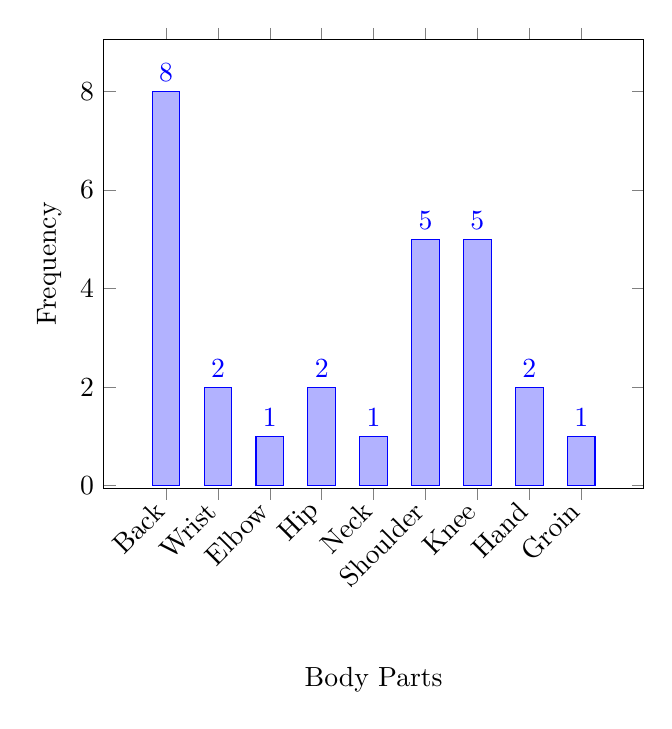
\begin{tikzpicture}
\begin{axis}[
    ybar,
    enlargelimits=0.15,
    ylabel={Frequency},
    xlabel={Body Parts},
    symbolic x coords={Back, Wrist, Elbow, Hip, Neck, Shoulder, Knee, Hand, Groin},
    xtick=data,
    nodes near coords,
    nodes near coords align={vertical},
    xlabel style={yshift=-20pt}, % Adjust the y position of the x-axis label
    x tick label style={rotate=45, anchor=east}, % Rotate x-axis labels
    ]
\addplot coordinates {(Back,8) (Wrist,2) (Elbow,1) (Hip,2) (Neck,1) (Shoulder,5) (Knee,5) (Hand,2) (Groin,1)};
\end{axis}
\end{tikzpicture}
        \end{center}

        \bigbreak \noindent 
        \textbf{Comparing Two Sets of Data}
        \bigbreak \noindent 
        First, determine the relative frequencies of each category for each year. To construct side-by-side bar graphs, draw two bars for each category of data.

        \bigbreak \noindent 
        \textbf{Horizontal Bars}
        \bigbreak \noindent 
        Bar graphs may also be drawn with horizontal bars. Horizontal bars are preferable when category names are lengthy. For example, Figure 4 uses horizontal bars to display the same data as in Figure 3.

        \bigbreak \noindent \bigbreak \noindent 
        \textbf{\textit{\underline{Construct Pie-Graphs}}}
        \bigbreak \noindent 
        Pie charts are typically used to present the relative frequency of qualitative data. In most cases, the data are nominal, but ordinal data can also be displayed in a pie chart.

        \bigbreak \noindent 
        \textbf{When should a Bar Graph or Pie Chart be Used?}
        \bigbreak \noindent 
        Pie chart are useful for showing the division of all possible values of a qualitative variable into its parts.
        \bigbreak \noindent 
        However, because angles are often hard to judge in pie charts, they are not as useful in comparing two specific values of the qualitative variable. 
        \bigbreak \noindent 
        Instead, the emphasis is on comparing the part to the whole.
        \bigbreak \noindent 
        Bar graphs are useful are useful when we want to compare the different parts, not necessarily the parts to the whole.

        \bigbreak \noindent 
        Since bars are easier to draw and compare, some forgo pie charts in favor of Pareto charts when comparing parts to the whole.

        \pagebreak \bigbreak \noindent
        \subsection{2.2: Organizing Quantitative Data: The Popular Displays}
        \bigbreak \noindent 
        \textbf{\textit{\underline{Learning Objectives For This Section:}}}
        \begin{enumerate}
            \item \textbf{Organize Discrete Data in Tables}
            \item \textbf{Construct Histograms of Discrete Data}
            \item \textbf{Organize Continuous Data in Tables}
            \item \textbf{Construct Histograms of Continuous Data}
            \item \textbf{Draw Dot Plots}
            \item \textbf{Identify the Shape of a Distribution}
        \end{enumerate}
        \bigbreak \noindent 
        \textbf{Vocab:}
        \begin{itemize}
            \item A \textbf{histogram} is constructed by drawing rectangles for each class of data. The height of each rectangle is the frequency or relative frequency of the class. The width of each rectangle is the same, and the rectangles touch each other.
            \item \textbf{Classes: } The Categories in which data is grouped
            \item \textbf{lower class limit:} the smallest value within the class 
            \item \textbf{upper class limit:} the largest value within the class 
            \item \textbf{Class Width: }  is the difference between consecutive lower class limits.
            \item A table is \textbf{open ended} if the first class has no lower class limit or the last class has no upper class limit
            \item We draw a \textbf{dot plot} by placing each observation horizontally in increasing order and placing a dot above the observation each time it is observed.
            \item \textbf{uniform distribution:} frequency of each value of the variable is evenly spread across the values of the variable. 
            \item \textbf{bell-shaped distribution:} highest frequency occurs in the middle and frequencies tail off to the left and right of the middle.
            \item \textbf{skewed right:} the tail to the right of the peak is longer than the tail to the left of the peak
            \item \textbf{skewed left:} tail to the left of the peak is longer than the tail to the right of the peak.
        \end{itemize}


        \bigbreak \noindent \bigbreak \noindent 
        \textbf{\textit{\underline{Organize Discrete Data in Tables}}}
        \bigbreak \noindent 
        Use the values of the discrete variable to create the classes when the number of distinct data values is small. The approach to summarizing the data is similar to that of constructing frequency or relative frequency distributions from qualitative data where the categories of data are determined by the actual observations.

        \bigbreak \noindent \bigbreak \noindent 
        \textbf{\textit{\underline{Construct Histograms of Discrete Data}}}
        \bigbreak \noindent 
        The \textit{histogram}, a graph used to present quantitative data, is similar to the bar graph.
        \bigbreak \noindent 
        The value of each category of data (number of customers) is on the horizontal axis and the frequency or relative frequency is on the vertical axis. Draw rectangles of equal width centered at the value of each category. 


        \bigbreak \noindent \bigbreak \noindent \bigbreak \noindent \bigbreak \noindent \bigbreak \noindent \bigbreak \noindent \bigbreak \noindent \bigbreak \noindent \bigbreak \noindent \bigbreak \noindent \bigbreak \noindent 
        \begin{center}
            \textbf{Histogram (Left) vs Bar Graph (Right)}
        \end{center}
        \bigbreak \noindent \bigbreak \noindent 
        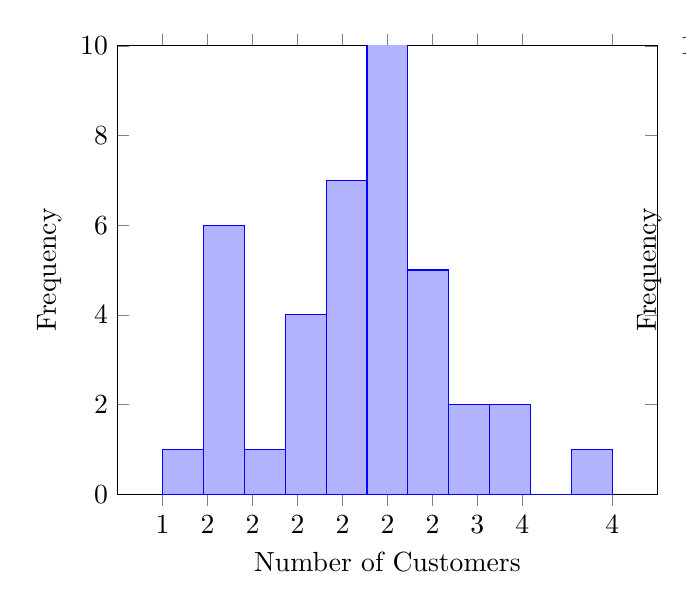
\begin{tikzpicture}
        \begin{axis}[
            ybar,
            ylabel={Frequency},
            xlabel={Number of Customers},
            ymin=0,
            ymax=10,
            xtick={1,2,3,4,5,6,7,8,9,11},
            xticklabels={1,2,2,2,2,2,2,3,4,4,4,4,5,5,5,5,5,5,5,6,6,6,6,6,6,6,6,6,6,7,7,7,7,7,8,8,9,9,11},
            enlarge x limits=0.1,
            ]
        \addplot+ [hist={bins=11}]
        table[row sep=\\,y index=0] {
        data\\
        1\\
        2\\
        2\\
        2\\
        2\\
        2\\
        2\\
        3\\
        4\\
        4\\
        4\\
        4\\
        5\\
        5\\
        5\\
        5\\
        5\\
        5\\
        5\\
        6\\
        6\\
        6\\
        6\\
        6\\
        6\\
        6\\
        6\\
        6\\
        6\\
        6\\
        7\\
        7\\
        7\\
        7\\
        7\\
        8\\
        8\\
        9\\
        9\\
        11\\
        };

        \end{axis}
        \hspace{3in}
        \begin{axis}[
            ybar,
            ylabel={Frequency},
            xlabel={Number of Customers},
            ymin=0,
            ymax=10,
            xtick=data,
            symbolic x coords={1,2,3,4,5,6,7,8,9,11},
            enlarge x limits=0.1,
            ]
        \addplot coordinates {
            (1,1)
            (2,6)
            (3,1)
            (4,4)
            (5,7)
            (6,10)
            (7,5)
            (8,2)
            (9,2)
            (11,1)
        };
        \end{axis}
        \end{tikzpicture}

        \bigbreak \noindent \bigbreak \noindent 
        \textbf{\textit{\underline{Organize Data Into Tables:}}}
        \bigbreak \noindent 
        When a data set consists of a large number of different discrete data values or when a data set consists of continuous data, create classes by using intervals of numbers.
        \bigbreak \noindent 
        \textbf{StatCrunch Steps:}
        \begin{itemize}
            \item Data $>$ Bin
            \item Select the column containing the data
            \item Choose a starting point and a binwidth (or automatic)
            \item Stat $>$ Tables $>$ Frequency (With newly generated data)
        \end{itemize}

        \bigbreak \noindent \bigbreak \noindent 
        \textbf{\textit{\underline{Draw Histograms of Continuous Data:}}}
        \bigbreak \noindent 
        \textbf{StatCrunch Steps:}
        \begin{itemize}
            \item Graph $>$ Histogram
            \item Select Data
            \item Input Bins
        \end{itemize}
        \textbf{Constructing Histograms Is Somewhat of an Art Form}
        \bigbreak \noindent 
        There is no one correct frequency distribution for a particular set of data. However, some frequency distributions better illustrate patterns within the data than others. So constructing frequency distributions is somewhat of an art form. Use the distribution that seems to provide the best overall summary of the data.
        \bigbreak \noindent 
         When the data set is small, we usually want fewer classes. When the data set is large, we usually want more classes. The larger the class width, the fewer the classes in a frequency distribution. Use the following guidelines to help determine an appropriate lower class limit of the first class and class width.

         \begin{mdframed}
             \textbf{\textit{\underline{Guidelines for Determining the Lower Class Limit of the First Class and Class Width}}}
             \bigbreak \noindent 
             \textbf{Choosing the Lower Class Limit of the First Class:}
             \bigbreak \noindent 
             Choose the smallest observation in the data set or a convenient number slightly smaller than the smallest observation in the data set.
             \bigbreak \noindent 
             \textbf{Determining the Class Width:}
             \begin{itemize}
                 \item Decide on the number of classes. Generally, there should be between 5 and 20  classes. The smaller the data set, the fewer the classes.
                 \item Determine the class width by computing
                     \begin{align*}
                         Class\ Width \approx \frac{Largest\ data\ value - smallest\ data\ value}{number\ of\ classes}
                     .\end{align*}
                \item Round the value to a convenient number. Rounding up may result in fewer classes than were originally intended, while rounding down may result in more class than originally intended.
             \end{itemize}
         \end{mdframed}

         \bigbreak \noindent \bigbreak \noindent 
         \textbf{\textit{\underline{Drawing Dot Plots:}}}
         \bigbreak \noindent 
         We draw a dot plot by placing each observation horizontally in increasing order and placing a dot above the observation each time it is observed.

         \bigbreak \noindent \bigbreak \noindent 
         \textbf{\textit{\underline{Identify the Shape of a Distribution:}}}
        \begin{figure}[ht]
            \centering
            \incfig{sr}
            \label{fig:sr}
        \end{figure}

        \pagebreak \bigbreak \noindent
        \subsection{2.4: Graphical Misrepresentations of Data}
        \bigbreak \noindent 
        \textbf{\textit{\underline{Learning Objectives For This Section:}}}
        \begin{enumerate}
            \item \textbf{Describe What Can Make a Graph Misleading or Deceptive}
        \end{enumerate}
        \bigbreak \noindent 
        \textbf{Vocab:}
        \begin{itemize}
            \
        \end{itemize}

        \bigbreak \noindent 
        \textbf{\textit{\underline{Describe What Can Make a Graph Misleading or Deceptive}}}
        \bigbreak \noindent 
        Statistics is the only science that enables different experts using the same figures to draw different conclusions.
        \bigbreak \noindent 
        Graphs that mislead unintentionally create an incorrect impression
        \bigbreak \noindent 
        Graphs that are deceptive purposely create an incorrect impression
        \bigbreak \noindent 
        \textbf{Most common graphical misrepresentations of data:}
        \begin{itemize}
            \item \textbf{Scale}
            \item \textbf{Inconsistent Scale}
            \item \textbf{Misplaced Origin}
        \end{itemize}
        \textbf{Guidelines for Constructing Good Graphics}
        \begin{itemize}
            \item Label and name the axes clearly, providing explanations if needed. Include units of measurement and a data source when appropriate.
            \item Include a meaningful title on the graph.
            \item Avoid distortion. Never lie about the data.
            \item Minimize the amount of white space in the graph. Use the available space to let the data stand out. If you truncate the scales, clearly indicate this to the reader.
            \item Avoid clutter, such as excessive gridlines and unnecessary backgrounds or pictures. Don't distract the reader from the data.
            \item Avoid three dimensions. Three-dimensional charts may look nice, but they distract the reader and often lead to misinterpretation of the graphic.
            \item Do not use more than one design in the same graphic. Sometimes graphs use a different design in one portion to draw attention to that area. Don't try to force the reader to a specific part of the graph. Let the data speak for themselves.
            \item Avoid relative graphs that do not contain data or scales.
            \item One final point to make. When reading graphs, look at the source of the data represented in the graphic. Often, a group with an agenda will conduct allegedly unbiased studies and report the results that support their position. Always "consider the source" and any possible hidden agendas they may have when reading graphics.
        \end{itemize}

    
\end{document}
